\documentclass[english]{article}
\usepackage[T1]{fontenc}
\usepackage[latin9]{inputenc}
\usepackage{float}
\usepackage{graphicx}
\usepackage{babel}
\begin{document}

\section{Driver disco ATA}

La implementación de driver $ATA$ que se implementó en este $SO$
permite acceso a un sector con offset y tamaño arbitrario (tanto para
lectura como para escritura). Si bien realizar esto, dificulto bastante
la lógica del driver, permite tener una logica de programación mas
simple en las capaz superiores ya que no es necesario leer un sector
entero para lugego ir hasta el offset deseado y obtener de ahi los
bytes deseados (ni hablar si se quiere tomar informaciòn que se encuentra
partida en varios sectores contiguos). Es por eso que el driver utilizado
permite $"abstraerse"$ de esta división por sectores y poder acceder
a disco a partir de un sector con cualquier offset y cualquier cantidad
de bytes que se quiera leer.

Además presenta otros métodos para detección de las propiedades de
un disco (Si es removible, ATA, soporta DMA y LBA), no se pudo (por
falta de tiempo) crear un comando para listar las cualidades de los
discos conectados desde las consolas, pero se espera poder mostrarlos
para la próxima entrega.

Un detalle a mencionar es que la escritura al disco con un offset
es muy cara ya que ATA solo permite escribir un sector entero, por
lo que para escribir un pedazo de uno de estos, primero hay que leerlo
entero en un buffer auxiliar, luego pisar los lugares a cambiar y
luego guardarlos, lo que seria equivalente a dos accesos a disco solo
para grabar una $x$ cantidad de bytes. Por lo que siempre se intenta
grabar la mayor cantidad de bytes posibles en cada acceso.

\pagebreak{}


\section{Disk Cache}

Debido a los problemas de eficiencia mencionados en la seccion anterior,
se decidió que seria una buena idea el tener una estructura cache,
que minimize los accesos a discos sin consumir mucha cantidad de moemria. 

La implementación de esta capa es muy sencilla, consiste en un vector
de $N$ estructuras en la que cada una tiene el contenido de un sector
entero y campos para indicar si el sector se encuentra sucio (necesita
ser escrito) y a que sector y disco corresponde.

El algoritmo de reemplazo elejido es el de LRU (es que menos accesos
tuvo, se reemplaza). 

Un problema al implementar esta capa era que hacer con los sectores
sucios ya que como se encuentran en RAM, hasta no ser guardados, la
informacion es propensa a perderse (ya sea por fallas del sistema,
corte de luz, etc). Frente a esto se decidió que cada una cantidad
fija de $ticks$, todos los sectores sucios serian escritos a disco. 

\pagebreak{}


\section{File System\protect \\
}

Nuestro File System se divide en dos partes, la primer parte es, el
file system en si y la segunda es la administracion de la infomacion
en el disco duro (DiskManager).

Para el manejo de archivos en $RAM$ de decidió tomar la misma implementacion
que usa Linux. Es decir, archivos regulares, directorioes, symbolic
links, etc son todos de tipo $fs$\_$node$ y lo único que los diferencia
es su campo $mask$ (en donde se define el tipo). Inicialmente se
comenzó tratando a cada tipo de archivo como un tipo de estructura
diferente, pero nos dimos cuenta que se volvía muy compleja la logica
de parseo de informacion en el disco.


\subsection{Manejo de disco}

Debido a la notable lentitud que posee el acceso a disco frente el
acceso a memoria, se diseñó el almacenamiento de la información teniendo
siempre en cuenta la cantidad de accesos y no tanto la cantidad de
bytes extras que se pueda llegar a desperdiciar por archivo.

Uno de los primeros problemas que se presentaron al comenzar a trabjar
en disco, era como averiguar si un determinado sector de memoria estaba
era o no valido. Frente a esto, en cada Header(mas adelante se hablara
mejor de estos) se agregó un campo $magic$ que sirve para validacion
de los campos leidos. En otras palabras, si el magic number coincide
con el magic number definido en el SO, entonces exite una estructura
valida almacendada en esa porcion de memoria. \\


El disco duro para este file system fue dividido basicamente en cuatro
sectores:
\begin{enumerate}
\item File System header
\item Memory bitmap
\item Vector de iNodos
\item Archivos
\end{enumerate}
\begin{figure}[H]
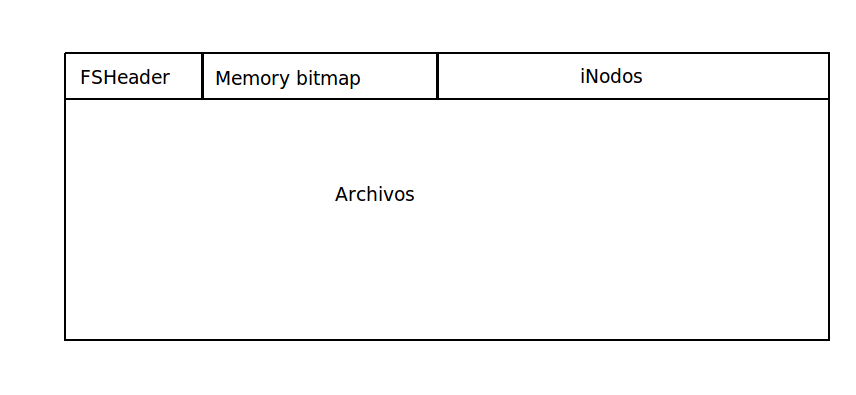
\includegraphics[width=10cm,height=5cm,keepaspectratio]{Imagen_disco}

\caption{Imgen disco duro}
\end{figure}


Para el F.S. Header simplemente se guardo un magic number y dos numeros
mas para indicar el tamaño maximo del vector de inodos y la cantidad
actual que existen. Esto es así ya que (por falta de tiempo), cada
vez que se crea un nuevo archivo, se consulta este valor, se lo incrementa
y luego se utiliza el valor obtenido para utizar la posicion $i-esima$
del vector de inodos (para el nuevo archivo). Se quiere aclarar que
esta es una implementación que nos parece muy mala y la que se tenía
pensado en utilizar una basada en bitmap, en donde el bit $i-esimo$
indicaria si el sector esta libre o no (este mismo algoritmo se utilizó
para el manejo de espacio en el disco duro y se explica en detalle
mas adelante). 

Cuando el SO se inicializa, intenta leer este sector de memoria, si
el magic number es valido, quiere decir que exite una particion valida
y entonces se intenta cargarla.

En cuanto al vector de iNodos, se trata de un vector de $N$ estructuras
de tamaño fijo (muy importante!) ya que permite el acceso al elemento
$i$ mediante una simple operacion matematica. En una de estas estructiras
del vector, se tiene almacenda una estructura de tipo $DiskPage$
(parte tres del disco), para indicar en que bloque del disco puede
la informacion ser encontrada y dos enteros, para indicar la cantidad
de bloques que esta página tiene reservada para su uso y otro para
la cantiad de bytes utlizados por el contenido del usuario.

La parte del disco dedicada a archivos se encuentra dividida en bloques
de tamaño fiijo definido por el SO. Lo mas importante para destacar
en esta parte es la forma que se tiene para el almacenamiento de cada
archivo. El formato elejido para el almacenamiento de la informacion
es muy parecido al de una $LinkedList$. Todo archivo en disco consiste
de:
\begin{enumerate}
\item Disk Page
\item File Header
\item Su contenido
\end{enumerate}
\begin{figure}[H]
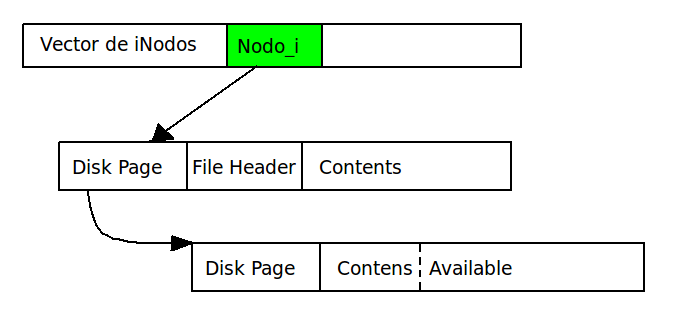
\includegraphics[width=10cm,height=7cm,keepaspectratio]{Archivo}

\caption{Formato de almacentamiento de un archivo}


\end{figure}


La estructura $File$$Header$ se guarda una única vez por cada archivo
y es la que posee el nombre, tipo, permisos y demás atributos que
no son parte del contenido en si.\\


Para crear un nuevo archivo, debe reservarse una determianda cantidad
de bloques. El primer algorimto que se utilizó para este trabajo consisitia
en ir leyendo cada bloque del disco desde el principio y utilizar
apartir de ahi los que necesito y esten diponibles. Inicialmente parecia
funcionar bien (ya que no se tenias mas de 2 o 3 carpetas creadas),
pero, a medida que se empezó a avanzar con el $SO$ y se requeria
de mayor catidad de archivos y carpetas, se comenzaba a ver lo terriblemente
lento que podia volverse este algoritmo. Es en esta parte donde entra
en uso el sector de $memory$ $bitmap$, el cual se ecuentra complentado
todo el sector 0 del disco duro (al lado del FS header). Cada bit
de esta porcion de memoria, indica si el bloque $i$ de la parte de
archivos se encuentra ocupada o libre. De esta manera, reservar bloques
siguie siendo de orden n pero con la importantisima diferencia que
solo se escribe cada sector a utilizar y no se lee mas que uno solo
(para escribir el header del sector recien reservado).


\subsection{Manejo en RAM}

El manejo de inodos es ram es bastante sencillo, el $FS$ mantiene
un vector con los últimos inodos consultados y ofrece la interfaz
para el SO para la modificiacion y consulta de estos ulimos en disco.
Cada vez que un nuevo inodo es consultado, se toma la siguiente posicion
de vector y se carga allí la información de disco de este inodo para
luego retornarla.

Un detalle a tener en cuenta es que esta implementación de $FS$ no
guarda ningún contenido de archivos (cache), ya que consideramos que
eso debía que ser trabajo de una entre el $diskManager$ y el driver
de disco ($diskCache$).

\pagebreak{}


\section{Problemas y posibles soluciones}

Uno de los problemas mas importantes que tiene esta implementacion
del $SO$ es la falta de semaforos y mutexes, especialmente para el
momento de reserva de memoria para archivos y para la lectura/escritura
de archivos! (problema de los N lectores y un escritor). Queda en
la lista de cosas para agregar en futuras actualizaciones del SO ya
que no pudo ser agregado por falta de tiempo. 
\end{document}

